\documentclass[12pt,fleqn]{article}\usepackage{../common}
\begin{document}
Paralel Rasgele Izdusumu

Rasgele yansitma teknigi $m \times b$ boyutunda bir matrisi $n \times
k$ boyutunda ve her hucresinde $N(0,1)$ dagilimindan gelen bir sayi
iceren matris ile carpmak sonunda elde edilir. Boylece ana veri
matrisi "yansiltilmis" olur, boyut azaltmak icin cok kullanisli bir
tekniktir, cunku elde edilen matrisin ana matris $A$'nin "menzilini"
iyi temsil ettigi ispatlanmistir. Daha fazla detay icin {\em Rasgele
Izdusumu ile SVD} yazisina bakabilirsiniz.

Esle/indirge ortaminda rasgele yansitma icin once {\em Matris
Carpimi} adli yaziya da bakmak gerekebilir. Bu yazida iki matris
arasindaki carpima "satir bakisi" bizim icin gerekli. Cunku carpimin
solunda $m \times n$ boyutundaki matrisin verileri bize satir satir
geliyor, yani her $m$ satirdan sadece bir tanesine bakarak islem
yapiyoruz. Faraziyemiz $n$'in de buyuk olabilmesine ragmen en azindan
$n$ tane veri noktasini tek bir makinada isleyebilecegimiz.

Satir bakisina donersek, bu carpim gorusune gore soldaki her satir
icin, o satirdaki bir ogeyi sagda ona tekabul eden $n \times k$
boyutundaki matrisin satiriyla (yani her gelen satirin 5. ogesi
sagdaki matrisin 5 satirin tamami ile) carpip, sonuc olan "carpilmis"
satirlari birbiriyle topluyoruz. Bu Hadoop veri isleme mentalitesine
uygun cunku her seferinde $A$'nin tek bir satirina bakiyoruz.

Sagdaki rasgele sayilar iceren matris kritik. Biz bu matrisi bellekte
tut\textbf{ma}maya karar verdik, cunku $n$ sayisi da buyuk olabilir, her
ne kadar $k$ kucuk olsa da (cogunlukla 100 civari) yine de bu kadar
bellegi eger mumkun ise israf etmemek en iyisi.

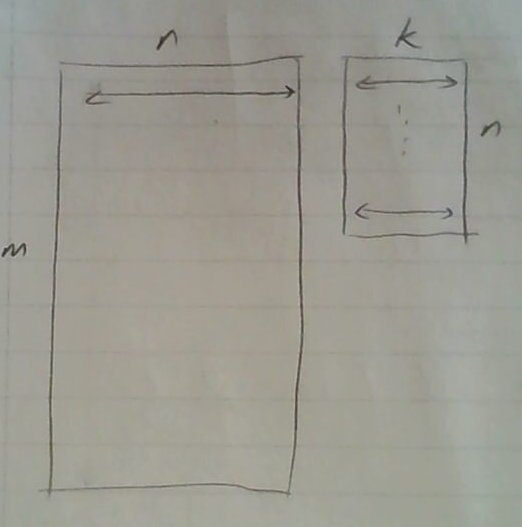
\includegraphics[height=6cm]{proj.png}


Eger bellekte tutmuyorsak rasgele matrisin degerlerini (sadece
ilgilendigimiz oge icin, tum matrisi degil) her seferinde tekrar
uretmek gerekir. Hiz acisindan performans cok kotu olmayacaktir, cunku
rasgele sayi uretimi toplama, carpma, $mod$ gibi direk matematiksel
hesaplar ile yapilir.

Fakat burada onemli bir diger konu sudur: her $A$ satiri icin {\em ayni}
rasgele matris (ogelerini) ayni sekilde uretebilmeliyiz.

Bu problemin en basit cozumu rasgele sayi uretimi icin tohum (seed)
kullanimidir. Eger tohum kullanilmazsa, Python \verb!random!
paketindeki uretici cagrilar gunun zamanina gore bir tohum
kullanirlar, ve boylece her cagri degisik bir sayi uretmis olur (cunku
komut isletildigi her seferinde gunun zamani degisiktir). Fakat
rasgele sayi uretimini, "her seferinde ayni sekilde" yaptirmanin yolku
vardir, bunun icin tohum disaridan set edilir ve boylece ayni tohumdan
baslayan rasgele sayi uretim zinciri hep ayni olur. Rasgele sayi
uretimi deterministik bir algoritmadir, zaten literaturde bu islem
"yari rasgele sayi uretimi (pseudorandom number generation)" olarak
gecer.

\begin{minted}{python}
import random

# tohumsuz, bu kod her seferinde degisik sayi uretir
print random.gauss(0,1), random.gauss(0,1)
print random.gauss(0,1), random.gauss(0,1)
\end{minted}

\begin{verbatim}
-0.49078710907 1.97156772689
-0.612135407803 -0.0159405924623
\end{verbatim}

\begin{minted}{python}
import random
# tohumlu
random.seed(100000)
print random.gauss(0,1), random.gauss(0,1)
random.seed(100000)
print random.gauss(0,1), random.gauss(0,1)
\end{minted}

\begin{verbatim}
1.46560757321 0.974749135866
1.46560757321 0.974749135866
\end{verbatim}

Ustteki kodda ayni tohumu verince arka arkaya uretilen iki (daha fazla
da olabilirdi) "rasgele" sayinin hep ayni oldugunu goruyoruz.

Rasgele "matrise" donersek, eger bu matrisin her $A$ veri satiri icin
hucre degerlerinin ayni sekilde uretilmesini istiyorsak, tohum
kullanmaliyiz. Tohum degeri ne olacak? Bu deger mesela $n \times k$
boyutundaki rasgele matris icin indis degerleri yanyana koyularak
uretilebilir, mesela 111. satir ve 2. kolon icin 1112 tohum degeri
kullanilir, ve bu tohumla tek bir rasgele sayi uretilir, (111,2)
hucresine konulur ve sonraki indis icin yeni bir tohum
kullanilir. Evet ust uste cakismalar olabilir tabii ki, mesela
11. satir 12. kolon da ustteki tohumla ayni sonucu getirir, ama bu tur
nadir cakismalar o kadar onemli degil, sonucta rasgele sayilarla
ugrasiyoruz, "yeterince raslantisal olmalari" kafi.

Altta bu veri matrisini satir satir carpip yansitilmis yeni bir
matrisi ureten mrjob programini bulabilirsiniz.

\inputminted{python}{mrproj.py}

Tek bir esle cagrisi var, cunku carpim islemi oldukca basit, indirgeme
islemine gerek yok.

Cikti icin yield ile yayinladigimiz (emit) satirlarda anahtar
kullanmiyoruz, yani verinin paralel islenirken nasil yuk dagitimi
yapildigina gore sonuc matrisinin sirasi ana matrisin satir sirasina
uymayabilir. Fakat satir sirasi bizim icin cogunlukla onemli olmuyor
(kolon sirasi onemli), cunku genelde, her satir, digerinden ayri /
bagimsiz bir veri olcumunu temsil eder cogunlukla. Eger zamansal bir
boyut var ise, bazi seyler arka arkaya islenmeliyse, o bilgi ayri bir
kolon (mesela tarih, zaman damgasi -timestamp-) olarak veride
bulunurdu.

\begin{minted}{python}
!python mrproj.py A_matrix > /tmp/out
\end{minted}

\begin{verbatim}
using configs in /home/burak/.mrjob.conf
creating tmp directory /tmp/mrproj.burak.20131203.094548.254606
writing to /tmp/mrproj.burak.20131203.094548.254606/step-0-mapper_part-00000
Counters from step 1:
  (no counters found)
Moving /tmp/mrproj.burak.20131203.094548.254606/step-0-mapper_part-00000 -> /tmp/mrproj.burak.20131203.094548.254606/output/part-00000
Streaming final output from /tmp/mrproj.burak.20131203.094548.254606/output
removing tmp directory /tmp/mrproj.burak.20131203.094548.254606
\end{verbatim}

\begin{minted}{python}
!head -10 /tmp/out
\end{minted}

\begin{verbatim}
20.2369671373,13.9358970644,0.524561578258
19.8581349841,13.7724732852,5.23992858318
27.6790861925,18.8833585029,-1.56199395804
9.3255498646,7.52383094482,2.58977793605
27.3677257439,33.0438553532,18.4819155509
27.6790861925,18.8833585029,-1.56199395804
9.3255498646,7.52383094482,2.58977793605
27.3677257439,33.0438553532,18.4819155509
27.6790861925,18.8833585029,-1.56199395804
9.3255498646,7.52383094482,2.58977793605
\end{verbatim}

Performans Iyilestirmeleri

Ustteki kod daha hizli olabilir. Diyelim ki $n$'in milyonlarda oldugu
sartlari da hizli bir sekilde isleyebilmek istiyoruz. Fakat bu noktada
kendimize su soruyu sormamiz gerekir: hangi sartlarda $n$ milyonlari
bulacaktir?

Buyuk bir ihtimalle bu durum eger bolca kategorik veri boyutu var ise
ortaya cikar. Kategorik verileri bildigimiz gibi 1-in-n, ya da one-hot
kodlama (encoding) ile temsil ediyoruz, bu demektir ki 1000 tane
farkli deger icerebilen tek bir kolon, 1000 tane yeni kolon haline
geliyor. Bazi boyutlarin (mesela web sayfa ismi, URL degeri) tasiyan
veri setlerinde tekil (unique) degerlerin milyonlar hatta milyara
varabilecegini dusunursek asiri yuksek $n$ rakamlarinin nereden
geldigini anlariz.

Ama bunun bize ek bir faydasi var: 1-in-n kodlamasi var ise, bu her
satirda cok fazla sifir olacak demektir, ve icinde cok sifiri olan
vektorleri / matrisleri seyrek matrisler ile cok rahat sekilde temsil
edebiliriz.

\inputminted{python}{mrprojs.py}

Ustteki kodda her satiri okur okumaz hemen onu bir seyrek matrise
ceviriyoruz. Simdi en kritik numara: \verb!itertools.izip!
cagrisi ile bu seyrek matrisin {\em sadece sifir olmayan degerlerini
ziyaret ediyoruz}. Eger 1000 tane kolon var ise, ama bu 1000
kolonun 20 tanesi dolu ise, bu 50 kat bir performans iyilestirmesi
saglayacak demektir (bu arada seyrek verilerde yuzde 2 doluluk gayet
normal bir rakamdir). Sadece dolu hucreleri ziyaret ediyoruz, ayrica
\verb!izip! bu dolu hucrelerin indis degerlerini de bize geri
getiriyor, biz de bu degerleri \verb!seed! icin onceden oldugu
gibi kullaniyoruz. Bir diger ilerleme $K$ tane rasgele sayiyi bir
kerede uretiyoruz, ve tohum ayarlamasini bir kere, dis dongu basinda
gerceklestiriyoruz. 

Sonuclara bakalim:

\begin{minted}{python}
!python mrprojs.py A_matrix > /tmp/out
!head -10 /tmp/out
\end{minted}

\begin{verbatim}
using configs in /home/burak/.mrjob.conf
creating tmp directory /tmp/mrprojs.burak.20131203.094635.908870
writing to /tmp/mrprojs.burak.20131203.094635.908870/step-0-mapper_part-00000
Counters from step 1:
  (no counters found)
Moving /tmp/mrprojs.burak.20131203.094635.908870/step-0-mapper_part-00000 -> /tmp/mrprojs.burak.20131203.094635.908870/output/part-00000
Streaming final output from /tmp/mrprojs.burak.20131203.094635.908870/output
removing tmp directory /tmp/mrprojs.burak.20131203.094635.908870
20.4375200961,1.09117093744,-9.27846872665
13.2830062024,-0.654868464606,-9.66445859893
26.4299520755,0.628144156713,-14.4142094864
9.52053667131,0.337287636006,-3.17826479151
34.6111912648,-0.763663777689,-2.06399979621
26.4299520755,0.628144156713,-14.4142094864
9.52053667131,0.337287636006,-3.17826479151
34.6111912648,-0.763663777689,-2.06399979621
26.4299520755,0.628144156713,-14.4142094864
9.52053667131,0.337287636006,-3.17826479151
\end{verbatim}

Daha onceki sonuclar ile ayni (rasgelelik var ama \verb!seed!
degerleri degismedi, o sebeple ayni sonucu aldik, bu iyi).

Bir kontrol daha var, eger rasgelelik bazli yansitma iyi yapildiysa, $A$
matrisini izdusumunu aldiktan daha once anlattigimiz teknik ile SVD
hesabini cok rahat bir sekilde yapabilmeliyiz. Bunun icin izdusumunu
\verb!/tmp/Y! icine yazacagiz, ve ardindan daha onceki QR bazli
teknikle SVD hesabini yapacagiz. Ardindan pur SVD ile $A$'yi isleyecegiz ve
sonuc $U$ matrisindeki en buyuk iki tekilsel (singular) degeri her iki
teknikten alip ekranda grafikleyecegiz.

\begin{minted}{python}
!python mrprojs.py A_matrix > /tmp/Y

import numpy as np
import numpy.linalg as lin
import matplotlib.pyplot as plt

n = 4; k = 3
A = np.loadtxt('A_matrix')
Y = np.loadtxt("/tmp/Y",delimiter=',')

Q, xx = lin.qr(Y)
B = np.dot(Q.T,A)
Uhat, Sigma, V = lin.svd(B)
U = np.dot(Q, Uhat)

plt.plot(U[:,0],U[:,1],'r+')
plt.hold(True)

U, Sigma, V = lin.svd(A);
plt.plot(U[:,0],U[:,1],'bx')
plt.savefig('rnd_1.png')
\end{minted}

\begin{verbatim}
using configs in /home/burak/.mrjob.conf
creating tmp directory /tmp/mrprojs.burak.20131203.094752.176690
writing to /tmp/mrprojs.burak.20131203.094752.176690/step-0-mapper_part-00000
Counters from step 1:
  (no counters found)
Moving /tmp/mrprojs.burak.20131203.094752.176690/step-0-mapper_part-00000 -> /tmp/mrprojs.burak.20131203.094752.176690/output/part-00000
Streaming final output from /tmp/mrprojs.burak.20131203.094752.176690/output
removing tmp directory /tmp/mrprojs.burak.20131203.094752.176690
\end{verbatim}

Sonuclar fena degil.

\end{document}
